\documentclass[a4paper,10.5pt]{article}
\usepackage[utf8]{inputenc}
\usepackage{amsmath}
\usepackage{wrapfig}
\usepackage{amssymb}
\usepackage{setspace}
\usepackage{bm}
\usepackage{tikz}
\usetikzlibrary{decorations.pathmorphing,decorations.markings}
\usepackage{float}
\usepackage{cite}
\usepackage{fancyhdr}
\usepackage{lastpage}
\usepackage{listings}
\usepackage{graphicx}
\usepackage{multicol}
\usepackage{enumitem}
\usepackage{color}
\renewcommand{\thefootnote}{\alph{footnote}}


\setlength{\textwidth}{16cm}
\setlength{\oddsidemargin}{0cm}
\setlength{\textheight}{23cm}
\setlength{\topmargin}{-1cm}
\setlength\parindent{0pt}
\renewcommand{\baselinestretch}{1.2}
\addtolength{\skip\footins}{7pt}

\pagestyle{fancyplain}
\lhead{}
\rhead{Tom Young 2021}
\cfoot{}
\lfoot{}


\begin{document}

\subsection{Gaussian Process Regression}

A Gaussian process (GP) is a collection of random variables such that any collection obey a multivariate normal distribution (MVN). Generally,
\begin{equation}
	\text{MVN} \sim \mathcal{N}(\boldsymbol{\mu}, \boldsymbol{\Sigma})
\end{equation}
is defined by its mean ($\boldsymbol{\mu} \in \mathbb{R}^d$) and covariance ($\boldsymbol{\Sigma} \in \mathbb{R}^{d \times d}$, positive semi-definite) for a $d$-dimensional distribution.%\footnote{The semi-definite requirement is because the PDF includes $\boldsymbol{\Sigma}^{-1}$.}

\begin{figure}[h!]
	\centering
	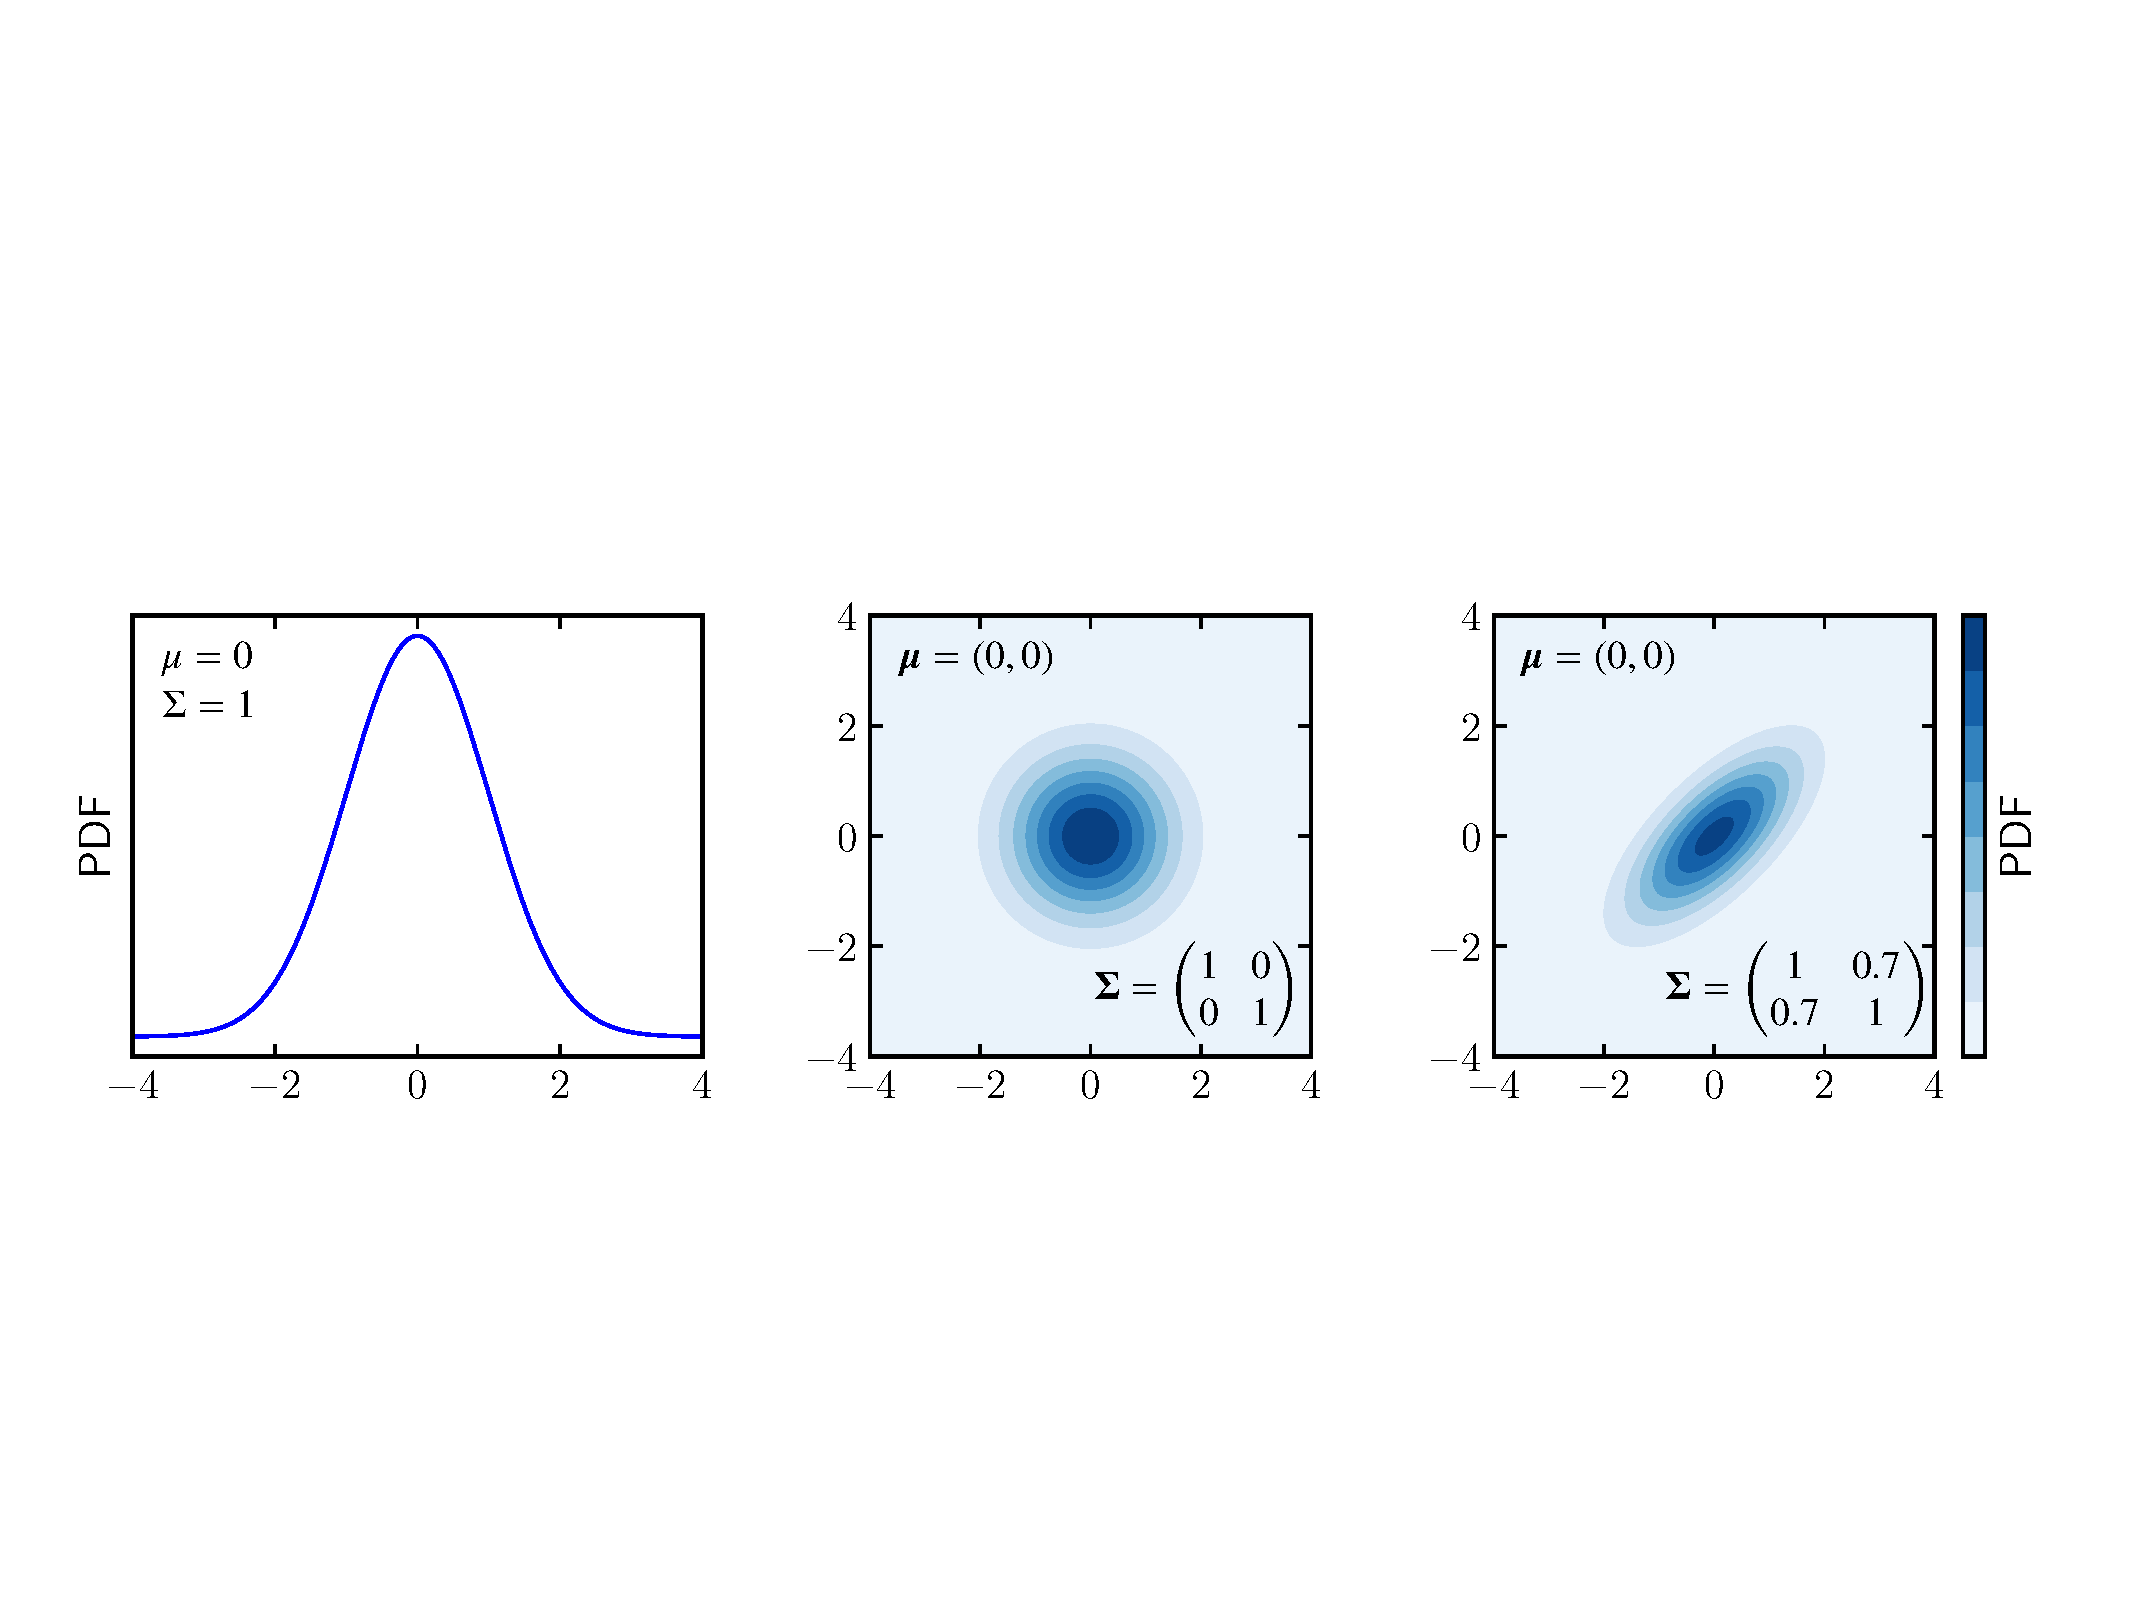
\includegraphics[width=\textwidth]{mvn_annotated.pdf}
	\vspace{0.1cm}
	\hrule 
	\caption{Various multivariate normal distributions in one and two dimensions.}
\end{figure}

To use a GP for regression the output ($y$) is defined in a linear way,
\begin{equation}
	y = \sum_i w_i \,\phi_i(\boldsymbol{x}) \equiv \boldsymbol{w}^T\tilde{\boldsymbol{x}}
\end{equation}
where $\boldsymbol{w}$ are the weights to be found and $\phi_i$ is a non-linear basis function of the input values ($\boldsymbol{x}$). The distribution of outputs and weights are set to be Gaussians,
\begin{equation}
	\begin{aligned}
		y^* &= \boldsymbol{w}^T\tilde{\boldsymbol{x}} + \varepsilon \qquad : \quad
		\varepsilon \sim \mathcal{N}(0, \sigma^2)\\
		w &\sim \mathcal{N}(0, c\mathbb{I})  \qquad\;\; : \quad c \in \mathbb{R}
	\end{aligned}	
\end{equation}
where the asterisk denotes a predicted value and $\boldsymbol{w}^T\tilde{\boldsymbol{x}} := z$ form the GP. 
\\\\
To do inference requires the posterior (predictive) distribution of $y$, given a set of known values. For the full set of $y$ then,\footnote{As the sum of independent MVNs just sum their means and covariances.}
\begin{equation}
	\begin{aligned}
		\boldsymbol{y} &= \boldsymbol{z} + \boldsymbol{\varepsilon} \\
		&\sim \mathcal{N}(\boldsymbol{\mu}, \mathsf{K} + \sigma^2\mathbb{I})
	\end{aligned}
\end{equation} 
defining $\mathsf{C} = \mathsf{K} + \sigma\mathbb{I}$ and splitting the vectors and matrices into known (train) and an unknown (${}^*$) components,
\begin{equation}
	\begin{pmatrix}
		y^*\\
		\boldsymbol{y}_\text{train}
	\end{pmatrix}
	\sim \mathcal{N}\left(
		\begin{pmatrix}
			\mu*\\
			\boldsymbol{\mu_\text{train}}
		\end{pmatrix}
	,
	\begin{pmatrix}
		\mathsf{C}^* & \mathsf{C}^*_\text{train} \\
		\mathsf{C}^{* T}_\text{train} & \mathsf{C}_\text{train}
	\end{pmatrix}
	\right)
\end{equation}

then the conditional distribution of $y^*$ is,

\begin{equation}
	(y^* | \boldsymbol{y}_\text{train}) \sim \mathcal{N}(\mu^* +  \mathsf{C}^{* T}_\text{train}\mathsf{C}_\text{train}^{-1}(\boldsymbol{y}_\text{train} - \boldsymbol{\mu}_\text{train})
	, \mathsf{D})
\end{equation}



\end{document}